% !TEX root = ../Dokumentation.tex
\subsection{Intelligente Systeme}

\subsubsection{Softwarekonzept}
\textbf{Funktionsbeschrieb}
\textbf{Komponentenbeschrieb}
\textbf{Begründung}
Wenn benötigt
\textbf{Berechnungen}
\textbf{Testergebnisse}

\subsubsection{Mini-Computer}
\textbf{Funktionsbeschrieb}
\textbf{Komponentenbeschrieb}
\textbf{Begründung}
Wenn benötigt
\textbf{Berechnungen}
\textbf{Testergebnisse}

\subsubsection{Mikrocontroller-Board}
\textbf{Funktionsbeschrieb}
Das Mikrocontrollerboard bildet die Schnittstelle zwischen der Hardware (Motor, Sensoren, Servos..) und dem Minicomputer. Das Mikrocontrollerboard übernimmt die Ansteuerung und Auswertung der einzelnen Komponenten und stellt die verarbeiteten Informationen dem Minicomputer über eine Schnittstelle zur Verfügung. \\
\\
\textbf{Komponentenbeschrieb}
\begin{figure}[h]
	\centering
	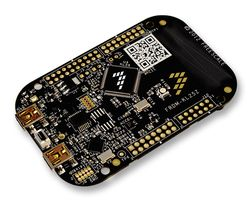
\includegraphics[width=0.5\textwidth]{./images/freedomboard.png}
	\caption{Freedomboard KL25 von Freescale (Quelle:http://ch.farnell.com/)}
	%http://ch.farnell.com/productimages/standard/de_DE/freescalesemiconductor-frdm-kl25z-40.jpg
\end{figure}
Als Mikrocontrollersystem wurde das Freedomboard KL25Z von Freescale ausgewählt. Das Etwicklungsgsboard bietet vieles, wie ausreichend I/O's, AD Wandler und Timerausgänge. Das Bord wird mit der Programmiersprache C programmiert. \\
\\
\textbf{Begründung}
Das Board überzeugt durch eine gute Rechenperformance zu einem kleinen Preis. Das Hauptargument für das Freedomboard ist die einfache Programmierung. Für viele Komponenten wie Servos oder Ultraschalsensoren steht ein Tool namens ProcessorExpert zu Verfügung. Diese Tool ermöglicht eine relativ einfache Anbindung solcher Komponenten. Dies spart sehr viel Entwicklungsaufwand.
Das Freedomboard hat sich gegen das Tinkerfogesystem durchgesetzt. Der Hauptgrund ist Flexibilität des Freedomboard gegenüber dem Tinkerfogesysem. Das Tinkerforgesystem ist sehr einfach zu bedienen solange alle Komponenten von Tinkerfogre zu Verfügung gestellt werden. Fehlt aber ein Modul wird es sehr schnell kompliziert. Beim Freedomboard ist der Aufwand für eine Komponente etwas höher, dafür können die meisten Systeme angeschlossen werden.\\
\\
\textbf{Testergebnisse}
Das Freedomboard wurde als Funktionsmuster bereits in Betrieb genommen. Es hat sich gezeigt, dass die Anbindung der Komponenten Tatsächlich sehr einfach ist. Es wurden bereits ein Ultraschallsensor, mehrere Servos, eine UART Kommunikation und ein Infrarotsensor angebunden. Das System sah dabei sehr vielversprechend aus.